% !BIB TS-program = biber 

\documentclass[12pt]{article}
\usepackage[margin = 1in]{geometry}
\usepackage{amsmath,amsfonts,graphicx,url,wrapfig,physics,caption}
\usepackage[colorlinks=true,plainpages=false,citecolor=blue,linkcolor=blue,urlcolor=blue]
{hyperref}
\usepackage{multirow}
\usepackage{caption}
\usepackage[calcwidth]{titlesec}

%%%%%%%%%% Bibliography stuff %%%%%%%%%%
\usepackage[style = ieee%,backend=biber,
]{biblatex}
\addbibresource{./bib.bib}

%%%%%%%%%% Title Page Preamble %%%%%%%%%%
\title{\textbf{Phys 295}}

\author{\noindent\rule{8cm}{0.4pt}\\
Rohith Vedhthaanth Sekar\\
TA: Peter Parker\\
Partners: Quinn Malin, Diego Martinez\\
Date: 04-Sep-2023\\
\noindent\rule{8cm}{0.4pt}
}



%%%%%%%%%% Begin the document %%%%%%%%%%

\begin{document}
\titleformat{\section}{\normalfont\bfseries}{\thesection.}{4 pt}{}
\captionsetup[figure]{labelfont={bf,footnotesize},labelformat={default},labelsep=period,name={Figure},font=footnotesize}


%%%%%%%%%% Making the title page %%%%%%%%%%
\makeatletter
\begin{titlepage}
\begin{center}
\vspace{1in}
\begingroup
\Large{\@title\\[0.5em]Lab report template}
\endgroup\\
\noindent\rule{16cm}{0.4pt}\\[10em]
\@author\\[1em]
\end{center}


%%%%%%%%%%  Here is the Abstract %%%%%%%%%%%%%%%
\begin{abstract}
This \LaTeX document sets out the basic structure of a report.  We will post the full sample report file after allowing time for the editing exercise.  The full file includes examples of equation typesetting, figure placement, and sub-sectioning. 
\end{abstract}
\end{titlepage}
\makeatletter


%%%%%%%%%%  Here is the Introduction %%%%%%%%%%%%%%%
\newpage
\section{Introduction}
Here are some citations to previous work~\cite{Dyson1920} and other work~\cite{Abbot2016}.


%%%%%%%%%%  Here is the Theory %%%%%%%%%%%%%%%
\section{Background/Theory}

A simple equation to calculate mean is given by:

\begin{equation} \label{eq:mean}
     \overline{x}=\frac{\sum_{i=i}^{n} x_{i}}{n} 
\end{equation}

When introducing an equation, it is important to define the variables used. For example, it is unclear what $n$ stands for in Eq.\ \ref{eq:mean} (note: a reference to the above equation is made here).


%%%%%%%%%%  Here are the Experimental Details %%%%%%%%%%%%%%%
\section{Experimental Details}

\begin{figure}[h!]
%\begin{wrapfigure}{l}{0.1\linewidth}
    \centering  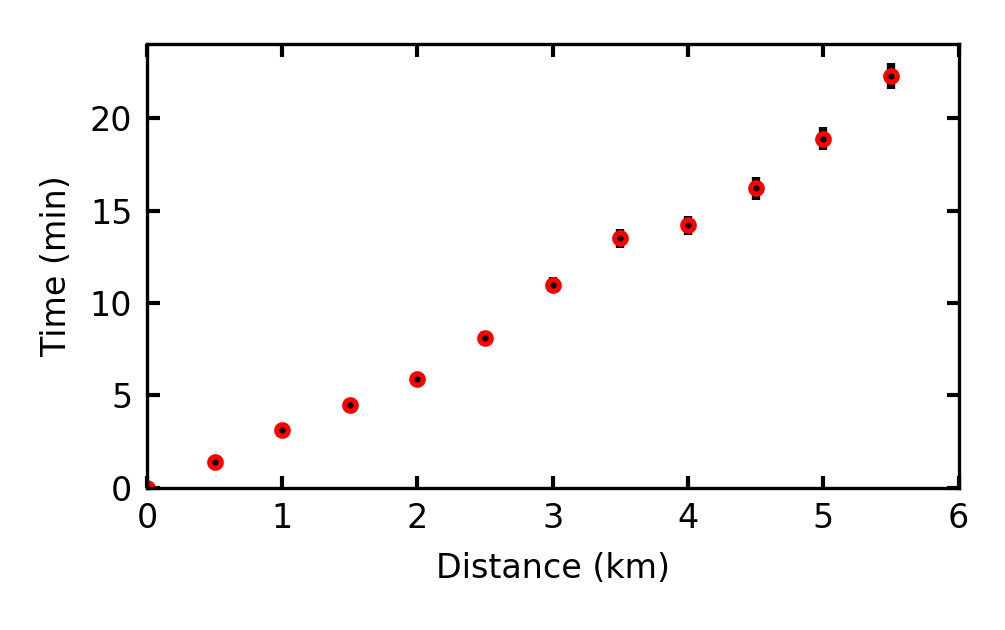
\includegraphics{BikeRidePlot.png}
  \caption{Measured time vs. distance for Lindsay's bike ride home one evening. Red points indicate measured times, with error bars indicating the estimated measurement uncertainty of each point (some error bars are smaller than marker size).}
  \label{fig:setup}
%\end{wrapfigure}
\end{figure}

The apparatus used in the CVGT experiment is the remnant of a mercury manometer equipped with an air-filled glass bulb placed inside a copper canister (see Fig.\ \ref{fig:setup}).  


%%%%%%%%%%  Here are the Results and Analysis %%%%%%%%%%%%%%%

\section{Results and Analysis}

Data is included in Table \ref{Data table} provided in the Appendix section.

%%%%%%%%%%  Here is the Discussion %%%%%%%%%%%%%%%
\section{Discussion}


%%%%%%%%%%  Here is the Conclusion %%%%%%%%%%%%%%%
\section{Conclusion}

%%%%%%%%%%  Here are the Acknowledgements %%%%%%%%%%%%%%%
\section{Acknowledgements}

%%%%%%%%%%  Here are the References (bibliography) %%%%%%%%%%%%%%%
\printbibliography

%%%%%%%%%%  Here is the Appendix %%%%%%%%%%%%%%%
\section*{Appendix}


\begin{table}[h!]
    \centering
    \begin{tabular}{ |c|c|c|c| } 
    \hline
    Voltage ($V$) & Current ($A$) & Resistance ($\Omega$) \\
    \hline
    V1 & A1 & R1 \\ 
    V2 & A2 & R2 \\ 
    V3 & A3 & R3 \\ 
    \hline
    \end{tabular}
    \caption{Data table}
    \label{Data table}
\end{table}

\noindent For more help with Equations, Figures, and Tables, see: 

\begin{itemize}
\item  \url{https://www.overleaf.com/learn/latex/Mathematical_expressions} (accessed 04 Sept 2023)
\item \url{https://www.overleaf.com/learn/latex/Inserting_Images}(accessed 04 Sept 2023) 
\item \url{https://www.overleaf.com/learn/latex/Tables} (accessed 04 Sept 2023).  
\end{itemize}

\end{document}
